\documentclass[msc,numbers]{coppe}
\usepackage{amsmath,amssymb}
\usepackage{hyperref}
\usepackage[latin1]{inputenc}
\usepackage[brazil]{babel}
\usepackage{graphicx}% Include figure files
\usepackage{multirow}
\usepackage{indentfirst}
\usepackage{subfigure}
\usepackage{url}
\usepackage{float}
\usepackage{textcomp}
\usepackage{tikz}
\usetikzlibrary{shapes,arrows}

\makelosymbols
\makeloabbreviations

\begin{document}
  \title{
    Intelig�ncia Computacional na Avalia��o de C�digos em um Sistema Complexo de Detec��o com Desenvolvimento Colaborativo
  }
  \foreigntitle{
    Computational Intelligence in Source Code Assertion in a Complex System in a Collaborative Development Enviroment
  }
  \author{Andressa A.}{Sivolella Gomes}
  \advisor{Prof.}{Jos�}{Manoel de Seixas}{D.Sc.}

  \examiner{Prof.}{Alu�zio Fausto Ribeiro Ara�jo}{D.Sc.}
  \examiner{Prof.}{Afonso de Bediaga e Hickman}{D.Sc.}
  \examiner{Pesquisadora}{Carmen L�cia Lodi Maidantchik}{D.Sc.}
  \department{PEE}
  \date{03}{2016}

  \keyword{Minera��o de c�digos}
  \keyword{M�todos ensemble com �rvores}
  \keyword{Plataforma colaborativa}

  \maketitle

  \frontmatter
  \dedication{A todo mundo, geralz�o.}

  \chapter*{Agradecimentos}

  Gostaria de agradecer a todos.

  \begin{abstract}

  Apresenta-se, nesta tese, ...

  \end{abstract}

  \begin{foreignabstract}

  In this work, we present ...

  \end{foreignabstract}

  \tableofcontents
  \listoffigures
  \listoftables
  \printlosymbols
  \printloabbreviations

  \mainmatter

  \chapter{Introdu��o}
    \section{Motiva��o}
    \section{Objetivos}
    \section{Organiza��o do documento}
  \chapter{A Colabora��o ATLAS do CERN}
    \section{CERN e LHC}
    Fundado em 1954, o CERN (em franc�s \emph{Centre Europ�en pour la Recherch� Nucl�aire}~\cite{CERN}) � o maior centro de pesquisa na �rea de f�sica de part�culas de altas energias no mundo. Atualmente, conta com a participa��o de 38 pa�ses membros e outros pa�ses colaboradores, entre eles o Brasil.

    O LHC (em ingl�s \emph{Large Hadron Collider}~\cite{LHC}) � o maior colisor de part�culas j� constru�do e encontra-se atualmente em opera��o no CERN. Instalado a 175 metros abaixo do solo, consiste em um grande t�nel em formato anelar, com 27 km de per�metro.
    \begin{figure}[htbp]
      \centering
        \includegraphics[width=9.0cm]{images/lhc-upper.png}
        \caption{Representa��o a�rea do LHC e seus detectores no CERN. Extra�do de~\cite{CDS}.}
      \label{LHC}
    \end{figure}
    Quando part�culas s�o eletricamente carregadas e submetidas a pulsos eletromagn�ticos no interior de tubos tem-se o processo de acelera��o de part�culas. Neste processo, as part�culas adquirem acelera��o ao serem envolvidas a campos eletromagn�ticos variantes~\cite{GRIFFITHS}. Em aceleradores circulares, part�culas s�o injetadas e circulam no anel at� atingirem a energia desejada. Diversos experimentos podem ser realizados em determinados pontos de colis�o ao longo da circunfer�ncia. O per�metro do acelerador circular � diretamente proporcional a energia necess�ria na colis�o. Ao atingir a energia desejada, os feixes de part�culas aceleradas em sentidos opostos colidem e, nesse caso, detectores em formato cil�ndrico s�o os mais utilizados. Cada colis�o gera informa��es que devem ser analisadas por especialistas, com objetivos distintos, tais como: identifica��o de sub-part�culas, observa��o de fen�menos e a comprova��o ou a elimina��o de teorias f�sicas. Nos pontos de colis�o, detectores s�o montados para observa��o e coleta de dados. Existem, por exemplo, detectores de calorimetria, para identificar a energia depositada pelas part�culas colisionadas; detectores de tra�os, para observar trajet�rias ap�s colis�es; e detectores de m�ons, respons�veis por absorver tais part�culas.


    A figura~\ref{LHC} ilustra uma representa��o a�rea do LHC. Existem quatro detectores de part�culas instalados em pontos de colis�o ao longo da extens�o do LHC, altamente especializados: ALICE~\cite{ALICE}, ATLAS~\cite{ATLAS}, CMS~\cite{CMS} e LHCb~\cite{SZUMLAK2010}.
    Os detectores ilustrados permitem obter informa��es detalhadas sobre a trajet�ria das part�culas resultantes das colis�es ocorridas e caracter�sticas energ�ticas, sendo poss�vel identificar part�culas. O ATLAS � o maior dos detectores do LHC.

    \section{Experimento ATLAS}
    O ATLAS (em ingl�s \emph{A Toroidal LHC AparatuS})~\cite{ATLAS} � um detector em formato cil�ndrico. O detector pesa aproximadamente 7.000 toneladas, com 44 metros de comprimento por 24 metros de altura. A figura~\ref{ATLAS} ilustra os diversos subsistemas que comp�em o detector ATLAS.

    Cada subsistema apresenta uma caracter�stica espec�fica de acordo com suas funcionalidades. S�o eles, da parte interna para a externa:
    \begin{itemize}
      \item{Detector Interno (ID)}, respons�vel por registrar as trajet�rias
        das part�culas resultantes da colis�o, bem como o momento e o sinal
        da carga, se for o caso;
      \item{Sistema de Calorimetria}, composto pelos calor�metros
        eletromagn�tico (LAr) e hadr�nico de telhas (TileCal). Os calor�metros citados s�o respons�veis por medirem a energia das part�culas resultantes;
      \item{Sistema Magn�tico}, respons�vel por desviar part�culas carregadas
        para medir o momento;
      \item{o Espectr�metro de M�ons}, respons�vel por medir a trajet�ria de
        uma determinada part�cula denominada M�on.
    \end{itemize}

    \begin{figure}[htbp]
      \centering
        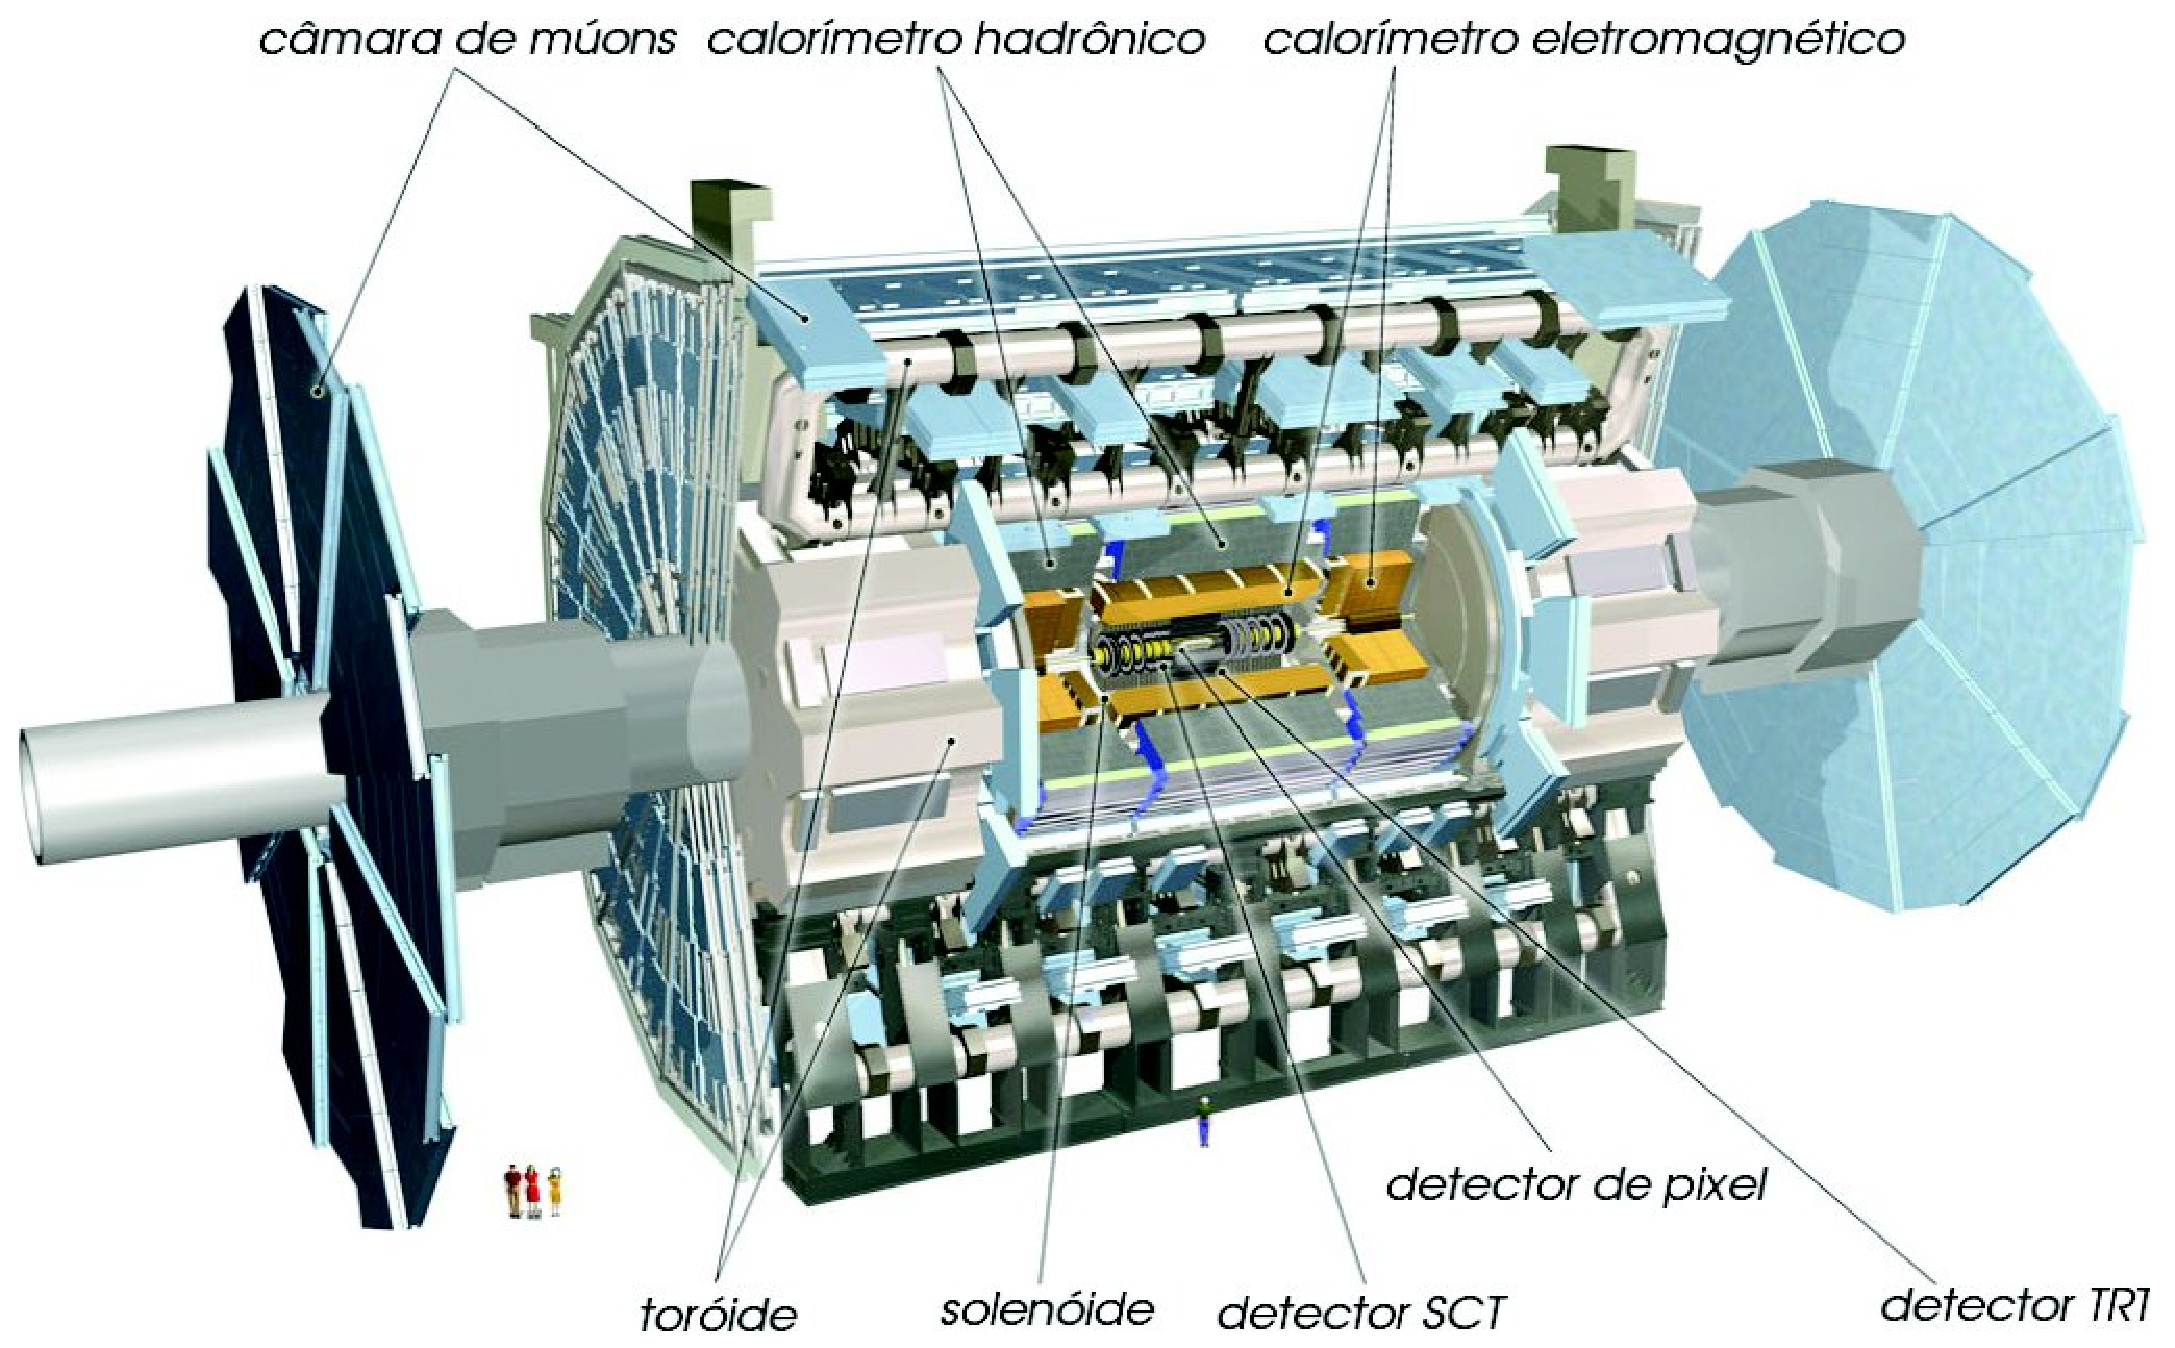
\includegraphics[width=12.0cm,height=8cm]{images/ATLAS_esquema.eps}
        \caption{Esquema do detector ATLAS. Adaptado de~\cite{ATLASPHOTOS}}
      \label{ATLAS}
    \end{figure}
    O sistema de calorimetria do LHC foi projetado para absorver a energia das part�culas que cruzam o detector, sendo o calor�metro hadr�nico de telhas (em ingl�s \emph{Tile Calorimeter} ou TileCal) � o foco deste mestrado.


    \section{Calor�metro Hadr�nico de Telhas (TileCal)}
        \subsection{An�lise \emph{Online} e \emph{Offline}}
        \subsection{A colabora��o TileCal}
  \chapter{Plataforma web Tile-in-ONE}
\label{tio}
Diversos sistemas foram desenvolvidos ao longo das diferentes fases do experimento, cada um com um prop�sito espec�fico~\cite{CHEP2010-DASHBOARD}. A an�lise \emph{online} tem in�cio com a aquisi��o e decis�o acerca do armazenamento dos dados adquiridos, que � responsabilidade do grupo TDAQ (do ingl�s, \emph{Trigger and Data Acquisition})~\cite{jenni2003atlas}. A reconstru��o dos dados pelo software para an�lise \emph{offline} ATHENA~\cite{ATHENA} marca o in�cio da an�lise \emph{offline}. Em seguida, o DQMF (do ingl�s, \emph{Data Quality Monitoring System})~\cite{DQMF} � aplicado e gera automaticamente estados para os PMTs, indicando a qualidade do tubo fotomultiplicador e reduzindo a quantidade de canais que precisam ser analisados. Nesta etapa, gr�ficos s�o gerados para auxiliar o grupo de qualidade de dados do TileCal em sua an�lise \emph{offline}. Um sistema web foi desenvolvido para integrar os resultados gr�ficos gerados durante a etapa de reconstru��o, guiando o grupo de qualidade de dados em suas an�lises. A figura~\ref{dashboard} ilustra sistemas integrados por uma �nica interface web: a figura~\ref{fig:dashboard_1} corresponde a lista de dados reconstru�dos e quais gr�ficos j� est�o dispon�veis para a colabora��o, indicando que a atua��o do ATHENA foi conclu�da; a figura~\ref{fig:dashboard_2} exibe informa��o detalhada sobre um determinado m�dulo, acessado pela interface ilustrada anteriormente. Atrav�s deste sistema web � poss�vel inserir coment�rios relacionados a performance do detector; e a figura~\ref{fig:dashboard_3} ilustra alguns gr�ficos gerados durante a etapa de reconstru��o dos dados.
\begin{figure}[!ht]
  \centering
  \subfigure[Lista dos dados adquiridos.]{
    \includegraphics[width=10cm]{images/screen-capture-5.png}
    \label{fig:dashboard_1}
  }
  \mbox{
    \subfigure[Estados gerados automaticamente pelo DQMF e acesso a informa��es detalhadas.]{
      \includegraphics[width=6.5cm]{images/screen-capture-6.png}
      \label{fig:dashboard_2}
    }
    \subfigure[Gr�ficos gerados para um determinado m�dulo.]{
      \includegraphics[width=6.5cm]{images/screen-capture-7.png}
      \label{fig:dashboard_3}
    }
  }
  \caption{\emph{Dashboard Web System}, desenvolvido em 2010 para integrar as os dados adquiridos e as an�lises do grupo de QD do TileCal. Mais detalhes em~\cite{CHEP2010-DASHBOARD}}
  \label{dashboard}
\end{figure}

Para uma refer�ncia hist�rica, a lista de canais definidos como defeituosos pela colabora��o (\emph{Bad Channels List}) � armazenada no banco de dados de condicionamento, comum a todos os experimentos que comp�em o LHC, o COOL DB~\cite{COOL_DB}. Os sistemas MCWS (do ingl�s, \emph{Monitoring \& Calibration Web System})~\cite{MCWS-CHEP-2012} e DCS (do ingl�s, \emph{Detector Control System})~\cite{DCS-CHEP-2009} apoiam o grupo de qualidade de dados na an�lise dos quase 10.000 PMTs do calor�metro de telhas. O MCWS foi desenvolvido para exibir a lista de canais defeituosos de maneira gr�fica e permite que coment�rios sobre o estado do detector sejam compartilhados. O sistema web DCS foi desenvolvido para monitorar as fontes de alta tens�o que alimentam os PMTs.

� evidente que o cen�rio descrito � composto por diversas ferramentas (web) para apoiar em diferentes aspectos as an�lises e opera��o de forma mais eficiente do TileCal. Tais sistemas foram desenvolvidos em diferentes fases do detector, envolvendo diferentes colaboradores, que n�o necessariamente ainda encontram-se envolvidos em atividades da colabora��o. Al�m disso, a manuten��o de tais ferramentas n�o � garantida pelos mesmos colaboradores contribuintes. Para a colabora��o, seria mais f�cil reunir todas as ferramentas existentes em uma �nica interface, que utilizasse preferencialmente a mesma tecnologia, permitindo inclusive, reutiliza��o de c�digos fonte. Tais requisitos foram contemplados com o projeto e desenvolvimento da Plataforma web Tile-in-ONE.

    \section{Fluxo de dados}

    A Plataforma Tile-in-ONE foi projetada para integrar as diferentes an�lises realizadas pela colabora��o TileCal. Ao fornecer uma estrutura onde os colaboradores podem desenvolver c�digos fonte diretamente atrav�s da web, ela integra diferentes ferramentas em um �nico lugar. Isso garante a escolha da mesma tecnologia para todas as ferramentas desenvolvidas (linguagem Python~\cite{PYTHON}), o que torna a manuten��o da plataforma mais f�cil. Al�m disso, existe o incentivo natural para reutiliza��o de c�digos, uma vez que os desenvolvimentos encontram-se dispon�veis para toda colabora��o. Outra funcionalidade oferecida pela plataforma � o encapsulamento em pacotes de configura��es para acessar bases de dados importantes para as an�lises. Isso permite que colaboradores novos n�o percam tempo aprendendo a acessar a informa��o, mas foquem na an�lise propriamente dita.

    A figura~\ref{fig:dataflow} ilustra o fluxo de dados do Tile-in-ONE. A plataforma oferece a funcionalidade de desenvolvimento de c�digos pela qual os colaboradores podem escrever seus pr�prios programas. Tamb�m � permitida a edi��o de c�digos salvos ou escritos por outros usu�rios. Uma vez que o desenvolvimento do c�digo � conclu�do, o desenvolvedor pode submeter seu c�digo que ser� manipulado no lado do servidor. Este, por sua vez, ir� direcionar o c�digo em quest�o para uma outra m�quina (nesse contexto, m�quinas \emph{slaves}), dependendo dos dados identificados pela plataforma que o c�digo fonte a ser executado deseja acessar. Cada m�quina \emph{slave} est� configurada para acessar um determinado reposit�rio de dados utilizado para as an�lises da colabora��o. Isso permite que os desenvolvedores se abstraiam de configura��es de acesso a tais reposit�rios. A motiva��o para efetuar a execu��o do c�digo fonte em outra m�quina que n�o no servidor � evitar que ocorra sobrecarga no servidor principal e o mais importante: caso o c�digo fonte falhe durante a execu��o, o servidor onde a plataforma est� hospedado n�o fica comprometido. A figura~\ref{fig:dataflow} ilustra ainda, em vermelho, onde esta tese de mestrado ir� atuar. O objetivo � criar uma etapa antes da submiss�o de novos c�digos para m�quinas \emph{slave}, atuando, desta forma, como uma camada de seguran�a cujo intuito � prever quais c�digos v�o falhar sem a necessidade de execut�-los. Esta camada consiste em um novo desenvolvimento e portanto, no momento, qualquer c�digo pode ser submetido para ser executado na m�quina \emph{slave}.

    Uma vez que o servidor web escolhe uma m�quina \emph{slave} esta tenta executar o c�digo fonte submetido e retorna para o servidor web, de maneira estruturada, o que ocorreu durante a execu��o. Neste momento, o desenvolvedor do c�digo fonte pode utilizar objetos gr�ficos tamb�m fornecidos pela plataforma para exibir os resultados recuperados atrav�s de seus c�digos fonte. Enfim, o c�digo fonte, a resposta obtida com a execu��o na m�quina \emph{slave} e os objetos gr�ficos s�o encapsulados em \emph{Plugins} e disponibilizados em \emph{Dashboards} para toda colabora��o.

    \section{Infraestrutura}

    A figura~\ref{fig:infrastructure} ilustra a infraestrutura atual da plataforma web Tile-in-ONE. Destaca-se em vermelho onde este mestrado pretende atuar.

    \begin{figure}[H]
      \centering
      \includegraphics[width=8cm]{images/infrastructure.png}
      \caption{Esquem�tico representando a infraestrutura da plataforma Tile-in-ONE. Em vermelho, a nova camada a ser desenvolvida.}
      \label{fig:infrastructure}
    \end{figure}

    \section{Novo desenvolvimento}

    A plataforma Tile-in-ONE est� atualmente sendo utilizada pelos grupos de calibra��o e qualidade de dados do TileCal. Uma preocupa��o que surgiu ao longo do ano de 2014 foi a execu��o bem sucedida de c�digos fonte sem avalia��o pr�via. Cada c�digo que enfrenta falhas durante sua execu��o na m�quina \emph{slave} acaba consumindo recursos computacionais que podem comprometer o fluxo de dados da plataforma como um todo. A solu��o para tal quest�o levantada � estudada neste mestrado, fazendo uso de t�cnicas de minera��o de c�digos fonte, como abordado no cap�tulo~\ref{code_mining}.

    \begin{figure}[H]
      \centering
      \includegraphics[width=7.5cm, height=24cm]{images/Tile-in-one_dataflow.png}
      \caption{Fluxo de dados da plataforma web Tile-in-ONE.}
      \label{fig:dataflow}
    \end{figure}
  \chapter{Minera��o de c�digos fonte para identifica��o de falhas}
    \section{Sele��o de categorias}
        \subsection{Analisadores Est�ticos}
        \subsection{Medidas estat�sticas e de qualidade}
    \section{Analisadores est�ticos e Minera��o de c�digos no CERN}
  \chapter{Metodologia}
\label{metodologia}
Este cap�tulo descreve o processo de estudo utilizado para este mestrado. 

As se��es~\ref{dataset} e~\ref{selection} descrevem, respectivamente, o conjunto de dados adquiridos e os atributos que foram previamente selecionados; A se��o~\ref{ensemble} descreve os algoritmos de m�quina de aprendizado utilizados;

    \section{Base de dados}
    \label{dataset}
    O Tile-in-ONE encontra-se em produ��o, sendo utilizado pelos grupos de calibra��o e qualidade de dados do TileCal desde 2014. Em seu banco de dados, existe um total de 512 c�digos de Plugins, desenvolvidos pelos colaboradores atrav�s da plataforma web. A figura~\ref{fig:developed_source_codes} corresponde a quantidade de c�digos fonte implementados no per�odo de Junho de 2014 a Dezembro de 2015.

    \begin{figure}[H]
      \centering
      \includegraphics[width=17cm]{images/total_source_codes.png}
      \caption{Total de c�digos fonte escritos (512) entre Junho/2014 e Dezembro/2015.}
      \label{fig:developed_source_codes}
    \end{figure}

    Dos 512 c�digos que comp�em o conjunto de dados, quase 30\% n�o obtiveram sucesso ao serem enviados para uma m�quina \emph{slave}. De acordo com a figura~\ref{fig:slave_machine_results}, percebe-se que 8,59\% n�o retornaram nenhum tipo de resposta para o servidor principal, o que pode significar que a m�quina \emph{slave} escolhida para executar o c�digo fonte em quest�o estava sem comunica��o. Isso n�o significa necessariamente que o c�digo fonte � \emph{n�o execut�vel}, uma vez que ele nem sequer chegou na m�quina \emph{slave}. Os 21,09\% restantes correspondem a programas que falharam durante a tentativa de execu��o. Mas novamente, n�o � poss�vel afirmar neste momento que tais c�digos s�o \emph{n�o execut�veis}. Se por ventura, algum desses tentou acessar um banco de dados (externo a plataforma) que no momento da execu��o estava inacess�vel, a m�quina \emph{slave} retornou falha e, neste caso, o problema n�o foi o c�digo fonte. Talvez no futuro, esse tipo de informa��o possa se tornar uma entrada para o classificador: caso o c�digo fonte esteja acessando uma fonte externa ele pode ser penalizado.

    \begin{figure}[H]
      \centering
      \includegraphics[width=8cm]{images/slave_machines_results.png}
      \caption{Retornos obtidos ap�s tentativa de executar c�digos fonte em m�quinas \emph{slave}.}
      \label{fig:slave_machine_results}
    \end{figure}

    Ap�s avaliar os 512 c�digos, e comparar com a aplica��o do analisador est�tico (PyLint), percebe-se que 82,02\% dos c�digos s�o \emph{execut�veis}, mas em quase 20\% dos casos o PyLint gera algum tipo de alerta. Do restante, menos de 1\% � \emph{n�o execut�vel} devido a erros de sintaxe em Python, mas podem ser facilmente identificados ao executar o analisador est�tico. Dos outros quase 17\% \emph{n�o execut�veis}, cerca de 5\% n�o podem ser identificados apenas com a aplica��o do Pylint. A figura~\ref{fig:targets} ilustra esses percentuais.

    \begin{figure}[H]
      \centering
      \includegraphics[width=8cm]{images/targets.png}
      \caption{Percentuais de alvos do conjunto de c�digos fonte.}
      \label{fig:targets}
    \end{figure}

    Em suma, a aplica��o do analisador est�tico n�o � suficiente para classificar um c�digo como \emph{execut�vel} ou \emph{n�o execut�vel}. Uma ferramenta adicional faz-se necess�ria.

    \section{An�lise de atributos}
    \label{selection}
    A tabela~\ref{tab:initialattributes} descreve os 11 atributos inicialmente extra�dos dos c�digos fonte dispon�veis na base de dados da plataforma Tile-in-ONE. Ao gerar a matriz de correla��o entre tais atributos (figura~\ref{fig:initialcorrelation}), percebe-se que os atributos relacionados �s medidas e estat�sticas de Halstead s�o fortemente correlacionados.

    \begin{figure}[H]
      \centering
      \includegraphics[width=10cm]{images/corr_matrix_11.png}
      \caption{Matriz de correla��o dos 11 atributos extra�dos inicialmente}
      \label{fig:initialcorrelation}
    \end{figure} 

    O teste $\chi^2$ foi aplicado para entender, dentre os atributos relacionados a Halstead, quais s�o os dois mais relevantes. Em outras palavras, dentre os atributos correlacionados, deseja-se utilizar os dois mais independentes, segundo o teste $\chi^2$. Para este caso, os atributos vencedores s�o: \emph{Halstead Volume} e \emph{Required Time}. A nova matriz de correla��o calculada (figura~\ref{fig:finalattributes}) demonstra que os 6 atributos selecionados (tabela~\ref{tab:finalattributes}) s�o suficientemente independentes entre si (com exce��o das medidas de Halstead). Observa-se ainda a independ�ncia dos atributos selecionados com o alvo, como ilustrado na figura~\ref{fig:finalattributes}.

    \begin{table}[]
    \centering
    \caption{Lista de atributos selecionados}
    \label{tab:finalattributes}
    \begin{tabular}{@{}|l|c|l|@{}}
    \toprule
    \multicolumn{1}{|c|}{\textbf{\#}} & \textbf{Atributo}                       & \multicolumn{1}{c|}{\textbf{Descri��o}}                            \\ \midrule
    1                                 & Complexidade Ciclom�tica                & N�mero de declara��es                                              \\ \midrule
    2                                 & �ndice de Manutenabilidade              & Corresponde � organiza��o do c�digo                                \\ \midrule
    3                                 & \multicolumn{1}{l|}{Volume de Halstead} & Combina��o entre n�mero de linhas e declara��es                    \\ \midrule
    4                                 & Tempo de Halstead                       & Tempo estimado para compilar um c�digo                             \\ \midrule
    5                                & LLOC                                    & N�mero de linhas l�gicas                                           \\ \midrule
    6                                & Alertas PyLint                          & \begin{tabular}[c]{@{}l@{}}Verdadeiro se PyLint gerou alertas. \\ Caso contr�rio, falso\end{tabular}\\ \bottomrule
    \end{tabular}
    \end{table}

    \begin{figure}[H]
      \centering
      \includegraphics[width=10cm]{images/finalattributes.png}
      \caption{Matriz de correla��o dos 6 atributos selecionados. As correla��es com a sa�da tamb�m s�o calculadas.}
      \label{fig:finalattributes}
    \end{figure} 

    \section{Classificadores em \emph{ensemble}}
    \label{training}

    Em F�sica de Altas Energias, � comum encontrar a aplica��o de BDT (\emph{Boosted Decision Tree}, ver se��o~\ref{bdt}) para identifica��o de part�culas. No Farmilab, por exemplo, as an�lises para busca de oscila��es de neutrinos deu-se por meio de aplica��o de BDT~\cite{Roe2005577}. No CERN existem diversos trabalhos utilizando BDT para identifica��o do B�son de Higgs. Portanto, existe um incentivo natural para a aplica��o de m�todos \emph{ensemble} com �rvores neste projeto contextualizado no ambiente do CERN. Como citado, a popularidade de �rvores de decis�o na comunidade cient�fica vem da sua f�cil compreens�o.

    Com os atributos selecionados (se��o~\ref{selection}), classificadores em \emph{ensemble} foram treinados. Para todos os casos, o algoritmo base � uma �rvore de decis�o, gerada previamente. O objetivo em se treinar mais de um classificador � avaliar se o problema a ser resolvido tem solu��o. Como sa�das, teremos as classes \emph{execut�vel} indicando que provavelmente o c�digo fonte n�o vai falhar ao ser executado na m�quina \emph{slave} ou, caso contr�rio, \emph{n�o execut�vel}.

    Antes de dividir o conjunto de dados em subconjuntos de treino (70\%) e teste (30\%), foi necess�rio replicar o conjunto com alvo \emph{n�o execut�vel}, devido a despropor��o em n�mero de amostras. � importante ressaltar que os mesmos conjuntos de treino e teste foram utilizados para todos os casos.

    Como avalia��o de performance, foram avaliadas as matrizes de confus�o e os F1-scores. Em an�lises estat�sticas de classifica��o bin�ria, o F1-score � uma medida de acur�cia. Ela considera tanto precis�o quanto sensibilidade, como pode ser observado pela f�rmula abaixo:

    \begin{center}
    $F1_{score} = 2 . \frac{p . r}{p + r}$
    \end{center}
    , onde $p$ � precis�o e $r$ � sensibilidade.

    Precis�o � o n�mero de verdadeiro positivos dividido pelo n�mero total de resultados positivos. Sensibilidade � o n�mero de verdadeiro positivos dividido pelo n�mero de resultados positivos que deveriam ter sido retornados.

    O F1-score pode ser interpretado como uma m�dia ponderada da precis�o e sensibilidade, onde o melhor valor para avaliar a acur�ria � 1 e o pior, 0.
    \\ \\
    \textbf{\large{�rvore de decis�o}}\\ \\
    O crit�rio \emph{gini} para divis�o da �rvore de decis�o foi utilizado. Estipulou-se um tamanho m�ximo igual a tr�s, a fim de evitar \emph{overfitting}. O esperado � que este classificador tenha uma acur�cia pior do que os demais. Esta �rvore foi utilizada como classificador base nos tr�s m�todos \emph{ensemble} utilizados descritos a seguir. 
    \\ \\
    \textbf{\large{Bagged Trees}}\\ \\
    Utilizando o mesmo conjunto de treino utilizado para treinar o classificador base e, utilizando a �rvore de decis�o descrita anteriormente, um classificador em \emph{Bagged Tree} foi gerado. No caso, o n�mero de itera��es estabelecido � igual a 100. Ou seja, ao final do treinamento, tem-se 100 �rvores treinadas. O resultado d�-se por voto majorit�rio dessas 100 �rvores. A cada rodada, 10\% do conjunto de treino foi utilizado como sub-conjunto \emph{boostrap} (o equivalente a cerca de 60 amostras). Isso � o suficiente para garantir que as amostras n�o sejam repetidas in�meras vezes, o que mant�m a independ�ncia dos 100 classificadores gerados pelo m�todo.\\ \\
    \textbf{\large{Random Forest}}\\ \\
    Para o classificador em \emph{Random Forest} os mesmos crit�rios estabelecidos para treinar o \emph{Bagged Tree} se aplicam. Mas, o que difere os dois m�todos � a quantidade de atributos utilizados em cada itera��o para treinar uma �rvore. Em~\cite{Breiman:2001:RF:570181.570182}, o Breiman avalia que empiricamente, um n�mero de atributos pr�ximo a $\sqrt{N}$ (sendo N o n�mero total de atributos) � suficiente para obter melhor acur�cia. No caso abordado nesta disserta��o, temos um n�mero de atributos pequeno (e igual a 6), de tal forma que $\sqrt{6} = 2.45$. O n�mero de atributos, ent�o, utilizado para treinar o classificador em \emph{Random Forest} � igual a 3. Como o \emph{OOB error} � calculado a cada itera��o, uma an�lise de relev�ncia de atributos tamb�m pode ser extra�da durante o treinamento deste classificador.\\ \\
    \textbf{\large{Boosted Decision Trees}}\\ \\
    Para treinar o classificador BDT o mesmo conjunto de treino foi utilizado. Existem diversos algoritmos que determinam como os pesos que ser�o atribu�dos �s amostras erroneamente classificadas em cada itera��o s�o definidos. No caso, o algoritmo \emph{AdaBoost}~\cite{Freund1997} (do ingl�s, \emph{Adaptative Boosting}) foi utilizado. Inicialmente, os pesos atribu�dos equivalem a 1. A cada itera��o o percentual de amostras classificadas de maneira equivocada � calculado e o peso que ser� atrib�ido a tais amostras � definido baseado neste percentual. O resultado final depender� tamb�m deste peso calculado a cada itera��o.

    A figura~\ref{fig:adaboost_pseudocode} ilustra um pseudo-c�digo extra�do de~\cite{Freund1997}. Nela � poss�vel entender como o peso $\beta$ � calculado, e tamb�m como o resultado final � obtido.

    \begin{figure}[H]
      \centering
      \includegraphics[width=8cm]{images/bdt_pseudocode.png}
      \caption{Pseudo-c�digo do algoritmo \emph{AdaBoost}}
      \label{fig:adaboost_pseudocode}
    \end{figure} 
  \chapter{Resultados e Conclus�es}
\label{resultados}
    \section{Avalia��o dos Classificadores}
    \label{avaliacao}
  \input{conclusao}

  \backmatter
  \bibliographystyle{coppe-unsrt}
  \bibliography{dissertacao}

  \appendix
  \chapter{Algumas Demonstra��es}
\end{document}